\chapter{\color{blue}Experimentos y resultados}\label{chapter5}

% **************************** Define Graphics Path **************************
\graphicspath{{Chapter5/Figs/}}


En este capítulo se muestran la experimentación y lo resultados obtenidos
que muestran la mejora en el desempeño de un agente que aprende
con y sin información adicional de un grafo causal.
Para mostrar que nuestro enfoque es una manera prometedora 
de mejorar el aprendizaje por refuerzo, se atacan dos problemas para
probar el concepto, la tarea de clásica del taxi \cite{Dietterich:2000:HRL:1622262.1622268} y la de los
interruptores de luz, descrita en el Capítulo \ref{chapter4}.
En resumen, los experimentos consisten en integrar el grafo $\mathcal{D}$ a la política $\epsilon$ greedy
en el algoritmo $Q$-learning \cite{watkins1992q}.
En la política $\epsilon$-greedy en vez de mantener fijo a $\epsilon$, se propone empezar motivando al agente a explorar y usar
el modelo causal e ir disminuyendo $\epsilon$ para dar más peso a la explotación.
Se comparan cuatro algoritmos, \textit{Q-learning sin información
adicional}, \textit{Q-learning con una estructural causal completa}, \textit{Q-learning con una estructura parcial} y un \textit{Q-learning con una estructura incorrecta}.
Cada uno de los algoritmos se ejecuta en una versión determinista y 
otra estocástica del ambiente. 
En las siguientes secciones se describen a detalle los experimentos realizados y los resultados. Todo el software desarrollado está 
disponible en \url{https://github.com/ivanfeliciano/causal_rl/}.


\section{Problema del taxi}

\subsection{Descripción de la tarea}

El primer problema a resolver es la tarea clásica del taxi \cite{Dietterich:2000:HRL:1622262.1622268}.
La Figura \ref{fig:taxi} muestra gráficamente el problema.
Existen cuatro posiciones en el mundo marcadas como R, B, G, y Y. 
La tarea es episódica. En cada episodio, 
el taxi comienza en un cuadro aleatoriamente elegido. 
Existe un pasajero en una de la cuatro posiciones (también elegida
aleatoriamente), y el pasajero desea ser transportado a una de las
cuatro zonas.
El taxi debe dirigirse a la posición del pasajero, recogerlo, ir a su destino y dejarlo.
El episodio termina cuando el pasajero es dejado en su destino.

\begin{figure}[H]
    \centering
    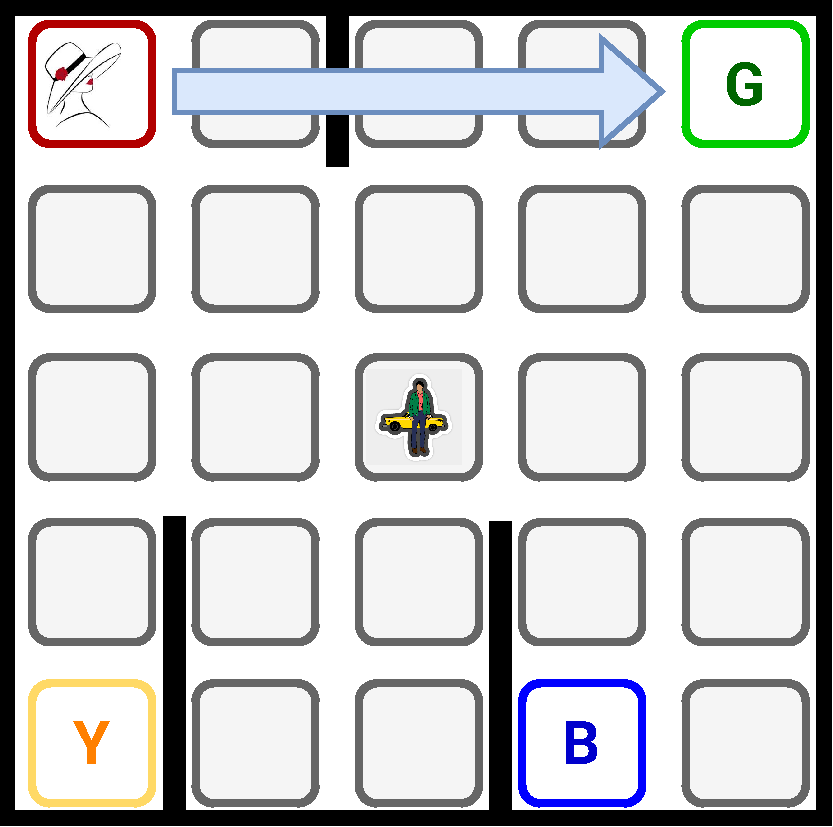
\includegraphics[scale=0.25]{Chapter5/Figs/taxi-env.pdf}
    \caption{La cuadrícula del ambiente del taxi. El taxi se encuentra en el cuadro central. En esta configuración del mundo, el objetivo es recoger al pasajero en la posición R y llevarlo a la posición G.}
    \label{fig:taxi}
\end{figure}

El conjunto de acciones $\mathcal{A}$ está compuesto por seis elementos: una acción para recoger $a_1$, una para dejar $a_2$ y
cuatro acciones de 
navegación que trasladan al taxi un cuadro al norte, sur, 
este u oeste, denotadas por $a_3, \dots, a_6$, respectivamente.
Existe una recompensa de -1 por cada acción, una recompensa adicional de 20 por cada pasajero llevado a su destino 
exitosamente y una penalización de -10 por acciones ilegales
de recolección y dejado.
El espacio de estados $\mathcal{S}$ tiene como elementos 
500 tuplas de tres elementos donde describen los 25 cuadros, las 5 posiciones del pasajero (incluyendo cuando está en el taxi) y los 4 destinos.


% Aquí ahondar más sobre el conjunto X y G, quienes lo compoenen y como está de pequeñito el problema
El conjunto $\mathcal{X}$ contiene 4 variables que traducen las tuplas con las posiciones del taxi y del pasajero en variables binarias. $x_1$
es la variable que dice si el taxi está en la misma posición que el
pasajero, $x_2$ es la variable que denota si el pasajero es llevado dentro del taxi, $x_3$ describe si el taxi está en la posición destino,
y $x_4$ es la variable que representa al estado de que el pasajero es entregado correctamente. Es una tarea relativamente simple y $x_1 \neq x_3$, por lo tanto las metas son $\mathcal{G} = \{\mathbf{g_1}, \mathbf{g_2}\}$, donde $\mathbf{g_1} = [1, 1, 0 , 0]$ y $\mathbf{g_2} = [0,1,1,1]$. La primera meta se puede ver como el sub objetivo de 
llevar subir al pasajero al taxi y la segunda meta es la general, 
entregar al pasajero en su destino.
El grafo causal $\mathcal{D}$ entre las variables de acción y los estados se puede 
ver en la Figura \ref{fig:cm-taxi}. Para este problema, los efectos
necesitan de todas sus causas para suceder, por ejemplo, para que el
pasajero esté dentro del taxi, $x_2 = 1$, entonces se debe actuar
subiéndolo al vehículo $a_1$ y además estar en la misma ubicación que
el pasajero.

\begin{figure}[H]
    \centering
    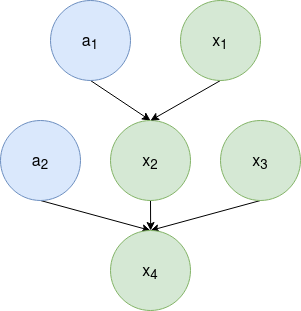
\includegraphics[scale=0.3]{Chapter5/Figs/causal_structure_taxi.png}
    \caption{Propuesta de una estructura causal para la tarea del taxi.}
    \label{fig:cm-taxi}
\end{figure}


\subsection{Configuración experimental}

Debido a la poca información que ofrece el grafo $\mathcal{D}$ y al tamaño de $\mathcal{G}$, para este problema no se ahonda en realizar experimentos con diferentes configuraciones. Por lo
tanto, sólo se comparan dos algoritmos,
el algoritmo Q-learning con y sin la estructura causal.
Además, los dos algoritmos se prueban sobre dos versiones del ambiente, una determinista
y otra estocástica. Los valores de los parámetros para los experimentos se muestran en la 
Tabla \ref{tab:tax-params}. Se ejecutan $M$ experimentos y cada experimento consiste de ejecutar cada algoritmo $k$ de episodios. La medida
de desempeño es la recompensa promedio por episodio. El valor de $\epsilon$ se va decrementando en cada paso de tiempo de entrenamiento $t$ de forma lineal ($\epsilon = \max(\epsilon_{\min}, mt + \epsilon_{\max})$, $m < 0$ y representa la tasa de decremento)
con respecto al
número de episodios, por lo que se fomenta la exploración y el uso del modelo causal al principio y posteriormente se explota la información de $Q$.

\begin{table}[H]
\centering
\caption{Parámetros para las versiones del algoritmo Q-learning.}
\label{tab:tax-params}
\begin{tabular}{ll}
\hline
Parámetro                                                                                      & Valor    \\ \hline
$\alpha$                                                                                       & 0.8      \\
$\gamma$                                                                                       & 0.95     \\
$\epsilon_{\min}$                                                                              & 0.1      \\
$\epsilon_{\max}$                                                                              & 1.0      \\
$m$                                                                                            & -0.0045 \\
$k$                                                                                            & 5000     \\
$M$                                                                                            & 10       \\
\begin{tabular}[c]{@{}l@{}}Probabilidad de\\ transición en ambiente\\ estocástico\end{tabular} & 0.7      \\ \hline
\end{tabular}
\end{table}

\subsection{Resultados}

En la Figura \ref{fig:results-taxi} se muestran los resultados obtenidos
para ambas configuraciones del ambiente (determinista y estocástico) donde los
los valores de los parámetros se describen en la Tabla \ref{tab:tax-params}.
La recompensa promedio por episodio para el método propuesto y para el algoritmo
original Q-learning están en color naranja y azul, respectivamente. 
Los resultados muestran que el algoritmo Q-learning guiado por el grafo da un salto inicial alto y mantiene una recompensa promedio mucho mayor que la versión sin información adicional. Esto era esperado, ya que 
no inicia una exploración a ciegas. Por otra parte, para el caso 
del ambiente estocástico, parecen comportarse de manera similar después de los
primeros 1000 episodios. Esto se puede deber a que tal vez la información del 
grafo no ayuda los suficiente, ya que a pesar de que tal vez existen
conexiones entre acciones y estados que no se están tomando en cuenta.


\begin{figure}[H]
  \centering
  \subfloat[Ambiente determinista.]{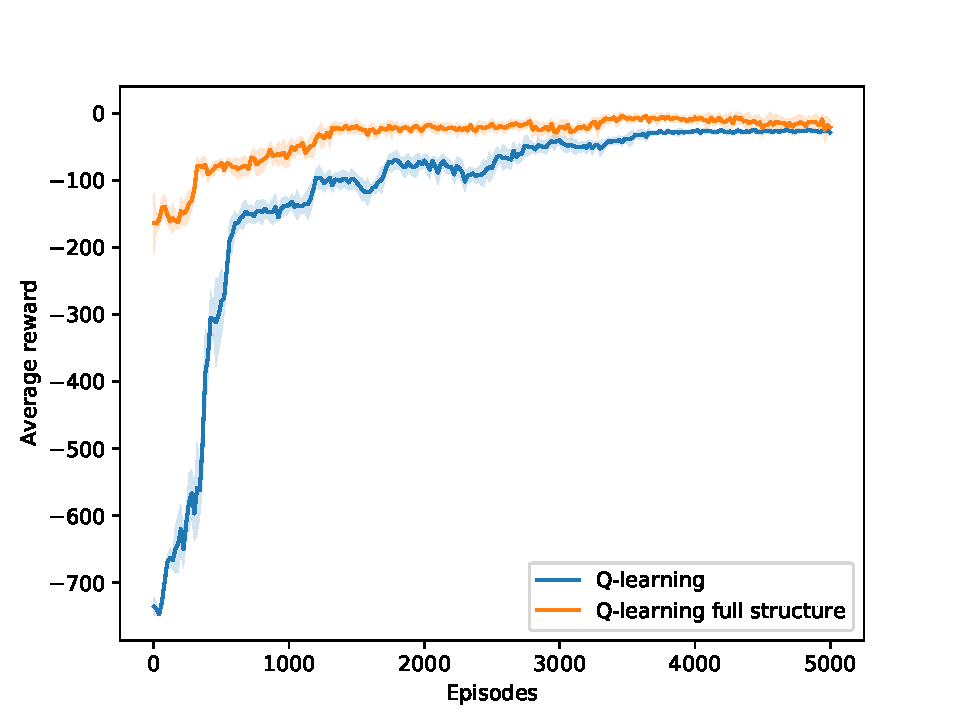
\includegraphics[width=0.5\textwidth]{Chapter5/Figs/taxiDet500010.pdf}\label{fig:taxi-rew-det}}
  \hfill
  \subfloat[Ambiente estocástico.]{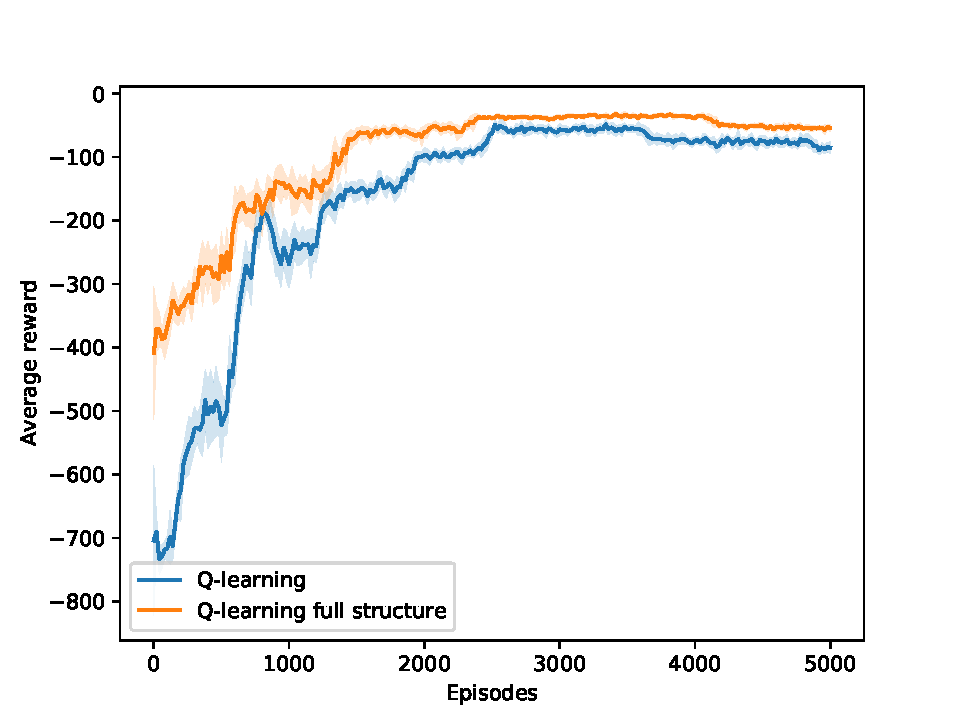
\includegraphics[width=0.5\textwidth]{Chapter5/Figs/taxiSto500010.pdf}\label{fig:taxi-rew-sto}}
  \caption{Comparación del desempeño para los dos algoritmos en 5000 episodios. La región sombreada es la desviación estándar para 10 experimentos.}
  \label{fig:results-taxi}
\end{figure}
\section{Problema de los interruptores de luz}

\subsection{Descripción de la tarea}
Para los experimentos de esta sección se ataca la tarea de control de interruptores de luz propuesta en \cite{nair2019causal} y descrita de manera general en la Sección \ref{section:switches-example}. Un agente tiene el control
de $N$ interruptores que controlan $N$ luces en un sitio.
Cada acción $a\in \mathcal{A}$ corresponde a mover un interruptor o 
a no mover ninguno, por lo tanto $|\mathcal{A}| = N + 1$.
El agente puede percibir dos tipos de señales del ambiente,
una imagen $s$ con una vista cenital del sitio, o vectores binarios $x \in \{0,1\}^N$ de 
macro-variables que codifican las luces prendidas, donde
$x_i = 1$ si la luz en la zona $i$ está prendida, de otro modo 
toma el valor $x_i = 0$.

Se exploran tres tipos de estructuras causales entre los
interruptores y las luces: \textit{uno-a-uno},
\textit{causa común} y \textit{efecto común}.
En los problemas con estructuras uno-a-uno cada interruptor corresponde a una sola luz.
Para el segundo tipo, de causa común, todas
las luces son controladas a lo más por un interruptor pero un
solo interruptor puede controlar más de una luz.
El tercer caso son estructuras de efecto común, donde cada interruptor
controla una sola luz, aunque múltiples interruptores
pueden controlar la misma luz. De manera visual, los tres tipos de estructuras
se muestran en la Figura \ref{fig:struct}.

\begin{figure}[H]
    \centering
    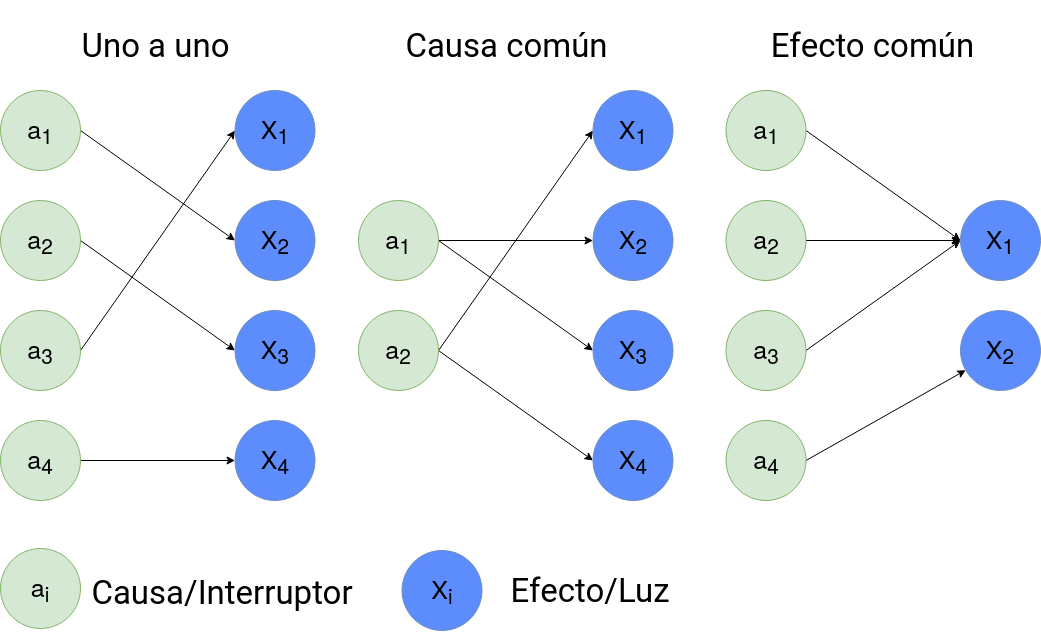
\includegraphics[scale=0.3]{Chapter5/Figs/switches_struct.png}
    \caption{Tipos de estructuras causales subyacentes posibles.}
    \label{fig:struct}
\end{figure}
La recompensa inmediata $r$ brindada al agente se calcula obteniendo la distancia entre el vector de variables de estado alto nivel $\mathbf{x}$ y el vector meta $\mathbf{g}$. En este problema se usa la distancia euclidiana.


\subsection{Configuración experimental general}

En las siguientes secciones se presentan experimentos para comparar el desempeño 
del método propuesto en diferentes escenarios, principalmente, para mostrar 
las posibilidades, ventajas y desventajas de usar un información del grafo causal, completa, incompleta e incluso incorrecta. A pesar de ser diferentes
experimentos se comparte la configuración para algunos elementos, por ejemplo, 
la medida de desempeño, el número de variables $N$, etc.

Se comparan cuatro algoritmos. Cada versión depende
de la cantidad y calidad de la información adicional con la que cuenta:

\begin{itemize}
    \item \textit{Q-learning sin información adicional}. Este método sirve como
    línea de base para medir que tanto mejora el aprendizaje. El algoritmo, dependiendo del espacio de estados sobre el que se trabaje, es el 
    algoritmo básico de Q-learning \cite{watkins1992q} o Q-learning profundo \cite{mnih2013playing}, para estados
    discretos y continuos, respectivamente. La selección de acciones se lleva a cabo mediante una política $\epsilon$ greedy clásica.
    \item \textit{Q-learning + estructura causal completa}. Durante la política de selección de acciones, el agente cuenta con la estructura causal del ambiente completa y verdadera $\mathcal{D}$.
    \item \textit{Q-learning + estructura causal incompleta}. En este caso el agente cuenta con un subgrafo $\mathcal{D'}$ del grafo $\mathcal{D}$. Este subgrafo se genera eliminando aristas de $\mathcal{D}$ aleatoriamente.
    \item \textit{Q-learning + estructura causal incorrecta}. Durante la política de selección de acciones, este algoritmo consulta un modelo $\mathcal{D}''$ con relaciones espurias y sin algunas relaciones verdaderas. Este grafo $\mathcal{D}''$ se obtiene generando un subgrafo de $\mathcal{D}$ como en el caso anterior y agregando aristas aleatoriamente.
\end{itemize}

\begin{figure}
  \centering
  \subfloat[$\mathcal{D}$.]{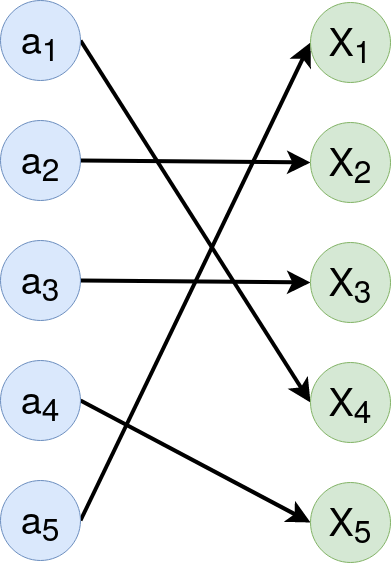
\includegraphics[width=0.2\textwidth]{Chapter5/Figs/completeD.png}\label{fig:completeD}}
  \qquad
  \subfloat[$\mathcal{D}'$]{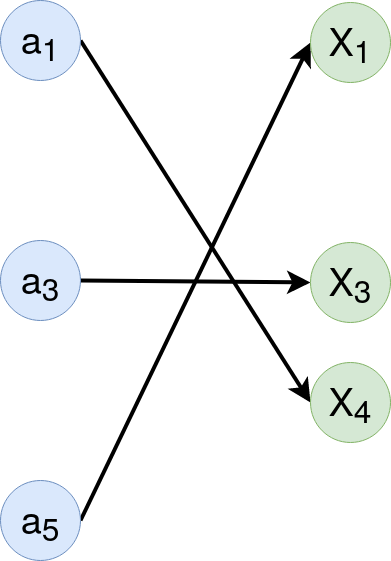
\includegraphics[width=0.2\textwidth]{Chapter5/Figs/incompleteD.png}\label{fig:incompleteD}}
%   \hfill
    \qquad
  \subfloat[$\mathcal{D}''$]{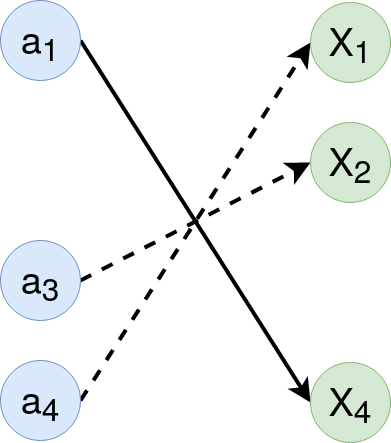
\includegraphics[width=0.2\textwidth]{Chapter5/Figs/wrongD.png}\label{fig:wrongD}}
  \caption{Ejemplo de los tres tipos de información con los que puede  contar el algoritmo Q-learning. El tipo de estructura
  del problema es uno-a-uno. Las aristas dirigidas punteadas describen conexiones espurias.}
  \label{fig:types-info-dag}
\end{figure}

Para medir el desempeño de los algoritmos se evalúa la recompensa
promedio sobre una serie de experimentos.
Cada experimento consiste en ejecutar el algoritmo de aprendizaje durante $k$ episodios, en 
un ambiente con una estructura causal fija $\mathcal{D}$ y donde se busca alcanzar la meta $\mathbf{g}$.
La recompensa promedio para el $i$ ésimo episodio está dada por
$R^{i} = \frac{1}{H}\sum_{t=0}^H r(\mathbf{x}_t, \mathbf{g})$,
donde $H$ corresponde al tamaño del episodio.
El vector $\mathbf{R_i}$, del $i$ ésimo experimento contiene las recompensas promedio por cada episodio, y se define como
$\mathbf{R_i} = (R^{1}, \dots, R^k)$.

Finalmente, la medida de comparación entre algoritmos es
el promedio de los vectores $\mathbf{R_i}$, $i\in [1, M]$,  obtenidos en $M$ experimentos. Esta medida, denotada como  $average$ puede escribirse como 
\begin{equation}
\label{eq:average}
average(\mathbf{R_1}, \dots, \mathbf{R_M}) = \frac{1}{M}(\sum^M_i \mathbf{R_{i}^1}, \dots, \sum^M_i\mathbf{R_{i}^k}),    
\end{equation}

donde $M$ es el número de experimentos y el $\mathbf{R_i^j}$ indica la recompensa promedio obtenida en el $j$ ésimo episodio del $i$ ésimo experimento.

El parámetro $\epsilon$ se disminuye linealmente, donde
en cada selección de acción va decreciendo hasta llegar
un valor mínimo. La regla de actualización de $\epsilon$ en
el paso de tiempo $t$ se puede definir como $\epsilon = \max(\epsilon_{\min}, -(\epsilon_{\max} - \epsilon_{\min}) \times t/ (N \times k) + \epsilon_{\max})$. Con excepción
del Experimento 2 (Sección \ref{subsection:exp-epsilon}), donde se cambia el denominador de la
tasa de decremento para que éste se más rápido.

Los experimentos se llevan a cabo en dos versiones del ambiente, una discreta y otra estocástica. Son tres los experimentos que se realizan. El primer experimento tiene 
como objetivo mostrar el comportamiento de modificar a
diferentes porcentajes la estructura causal $\mathcal{D}$ para obtener $\mathcal{D'}$ y $\mathcal{D}''$. El segundo experimento es con respecto a cambiar la tasa de decremento
de $\epsilon$ para llegar más rápido o lento a explotar 
más constantemente. El tercer experimentos, es probar
el algoritmo cuando no se tienen las variables
de alto nivel como observaciones directas, por lo tanto,
se trabaja sobre un espacio de estados continuo. En general,
algunos de los parámetros que se comparten entre los experimentos se muestran en la Tabla \ref{tab:switch-params}.

\begin{table}[H]
\centering
\caption{Valores para algunos parámetros de los algoritmos.}
\label{tab:switch-params}
\begin{tabular}{ll}
\hline
Parámetro                                                                                      & Valor    \\ \hline
$\alpha$                                                                                       & 0.8      \\
$\gamma$                                                                                       & 0.95     \\
$\epsilon_{\min}$                                                                              & 0.1      \\
$\epsilon_{\max}$                                                                              & 1.0      \\
$N$                                                                                            & \{5, 7, 9\} \\
$k$                                                                                            & \{200, 10000, 250000\}\\
$M$                                                                                            & 10       \\
\begin{tabular}[c]{@{}l@{}}Probabilidad de\\ transición en ambiente\\ estocástico\end{tabular} & 0.7      \\ \hline
\end{tabular}
\end{table}


\subsection{Experimento 1 - Cambios en el porcentaje de completitud de $D$}

\subsubsection{Configuración experimental}

\begin{itemize}
    \item  Lorem ipsum dolor sit amet, consectetur adipiscing elit. 
    \item Duis tincidunt placerat mollis. 
    \item Curabitur a turpis varius dui iaculis maximus vel ut lectus. 
    \item Donec mollis rutrum sapien et fringilla.
    \item Sed semper risus urna, id pretium libero vulputate vel. 
    \item Vivamus eu aliquam arcu. 
    \item Vivamus ornare risus augue, a efficitur massa iaculis eu. Nullam imperdiet facilisis tellus ut ullamcorper. 
\end{itemize}
\subsubsection{Objetivo}
\subsubsection{Hipótesis del experimento}
\subsubsection{Resultados}

Configuración low
\begin{figure}[H]
    \centering
    \includegraphics{example-image-a}
\end{figure}


Configuración medium
\begin{figure}[H]
    \centering
    \includegraphics{example-image-b}
\end{figure}

Configuración high
\begin{figure}[H]
    \centering
    \includegraphics{example-image-c}
\end{figure}

\subsubsection{Resultados}

Configuración low
\begin{figure}[H]
    \centering
    \includegraphics{example-image-a}
\end{figure}


Configuración medium
\begin{figure}[H]
    \centering
    \includegraphics{example-image-b}
\end{figure}

Configuración high
\begin{figure}[H]
    \centering
    \includegraphics{example-image-c}
\end{figure}




\subsection{Experimento 2 - Cambos en la tasa de consulta del modelo}\label{subsection:exp-epsilon}



\subsubsection{Configuración experimental}

\begin{itemize}
    \item  Lorem ipsum dolor sit amet, consectetur adipiscing elit. 
    \item Duis tincidunt placerat mollis. 
    \item Curabitur a turpis varius dui iaculis maximus vel ut lectus. 
    \item Donec mollis rutrum sapien et fringilla.
    \item Sed semper risus urna, id pretium libero vulputate vel. 
    \item Vivamus eu aliquam arcu. 
    \item Vivamus ornare risus augue, a efficitur massa iaculis eu. Nullam imperdiet facilisis tellus ut ullamcorper. 
\end{itemize}
\subsubsection{Objetivo}
\subsubsection{Hipótesis del experimento}
\subsubsection{Resultados}

Configuración low
\begin{figure}[H]
    \centering
    \includegraphics{example-image-a}
\end{figure}


Configuración medium
\begin{figure}[H]
    \centering
    \includegraphics{example-image-b}
\end{figure}

Configuración high
\begin{figure}[H]
    \centering
    \includegraphics{example-image-c}
\end{figure}

\subsubsection{Resultados}

Configuración low
\begin{figure}[H]
    \centering
    \includegraphics{example-image-a}
\end{figure}


Configuración medium
\begin{figure}[H]
    \centering
    \includegraphics{example-image-b}
\end{figure}

Configuración high
\begin{figure}[H]
    \centering
    \includegraphics{example-image-c}
\end{figure}



\subsection{Experimento 3 - Ambiente con estados continuos}


\subsubsection{Configuración experimental}

\begin{itemize}
    \item  Lorem ipsum dolor sit amet, consectetur adipiscing elit. 
    \item Duis tincidunt placerat mollis. 
    \item Curabitur a turpis varius dui iaculis maximus vel ut lectus. 
    \item Donec mollis rutrum sapien et fringilla.
    \item Sed semper risus urna, id pretium libero vulputate vel. 
    \item Vivamus eu aliquam arcu. 
    \item Vivamus ornare risus augue, a efficitur massa iaculis eu. Nullam imperdiet facilisis tellus ut ullamcorper. 
\end{itemize}
\subsubsection{Objetivo}
\subsubsection{Hipótesis del experimento}
\subsubsection{Resultados}

Configuración low
\begin{figure}[H]
    \centering
    \includegraphics{example-image-a}
\end{figure}


Configuración medium
\begin{figure}[H]
    \centering
    \includegraphics{example-image-b}
\end{figure}

Configuración high
\begin{figure}[H]
    \centering
    \includegraphics{example-image-c}
\end{figure}



\subsubsection{Resultados}

Configuración low
\begin{figure}[H]
    \centering
    \includegraphics{example-image-a}
\end{figure}


Configuración medium
\begin{figure}[H]
    \centering
    \includegraphics{example-image-b}
\end{figure}

Configuración high
\begin{figure}[H]
    \centering
    \includegraphics{example-image-c}
\end{figure}

\begin{itemize}

    \item Incluir toda la información necesaria para que el estudio
    pueda ser repetido.
    \item El propósito principal del reporte es diseminar los hallazgos o resultados.
    \item Tus hallazgos deben ser descritos con mucho detalle para que el lector los juzgue.
    \item Además debe haber suficiente detalle para hacer posible
    transferir cualquier solución a algún otro lugar.
\end{itemize}    


% \subsection{Esquemas de comparación}
% \subsubsection{Q-learning}
% \subsubsection{Q-learning con estructura causal completa}
% \subsubsection{Q-learning con estructura causal incompleta}
% \subsubsection{Q-learning con estructura causal incorrecta}
% \subsection{Parámetros y medidas de desempeño}

% \section{Resultados}
% \subsection{Ambiente con estados discretos}
% \subsubsection{Experimento 1 - Cambios en el porcentaje de la completitud de $D$}
% \subsubsection{Experimento 2 - Cambios en la tasa de consulta del modelo $\epsilon$}
% \subsubsection{Experimento 3 - Transferencia de conocimiento}
% \subsection{Ambiente con estados continuos}
% \subsubsection{Experimento 1 - Cambios en el porcentaje de la completitud de $D$}
% \subsubsection{Experimento 2 - Cambios en la tasa de consulta del modelo $\epsilon$}
% \subsubsection{Experimento 3 - Transferencia de conocimiento}

% \subsection{Q-learning}
% \subsection{Q-learning con estructura causal completa}
% \subsection{Q-learning con estructura causal incompleta}
% \subsection{Q-learning con estructura causal incorrecta}


